\documentclass[border=2pt]{standalone}
\usepackage[T1]{fontenc}
\usepackage{times}
\usepackage{pgfplots}
\usepgfplotslibrary{groupplots}
\pgfplotsset{compat=1.18}
\definecolor{cA}{HTML}{2A78D6}
\definecolor{cB}{HTML}{EB6834}
\definecolor{cC}{HTML}{1BAF7A}
\definecolor{cD}{HTML}{EDA100}
\definecolor{cGrey}{HTML}{6F7988}
\definecolor{cLight}{HTML}{AEB4BD}
\definecolor{cRule}{HTML}{D9DEE5}
\pgfplotsset{every axis/.append style={font=\footnotesize, axis line style={cGrey}, tick style={cGrey},
  major grid style={cRule, line width=0.3pt}, ymajorgrids, tick pos=left, label style={font=\footnotesize},
  title style={font=\footnotesize\bfseries, yshift=-2pt}, legend style={font=\scriptsize, draw=none, fill=none}},
  err/.style={error bars/.cd, y dir=both, y explicit, error mark options={rotate=90, mark size=1.5pt}, /pgfplots/.cd}}
\begin{document}
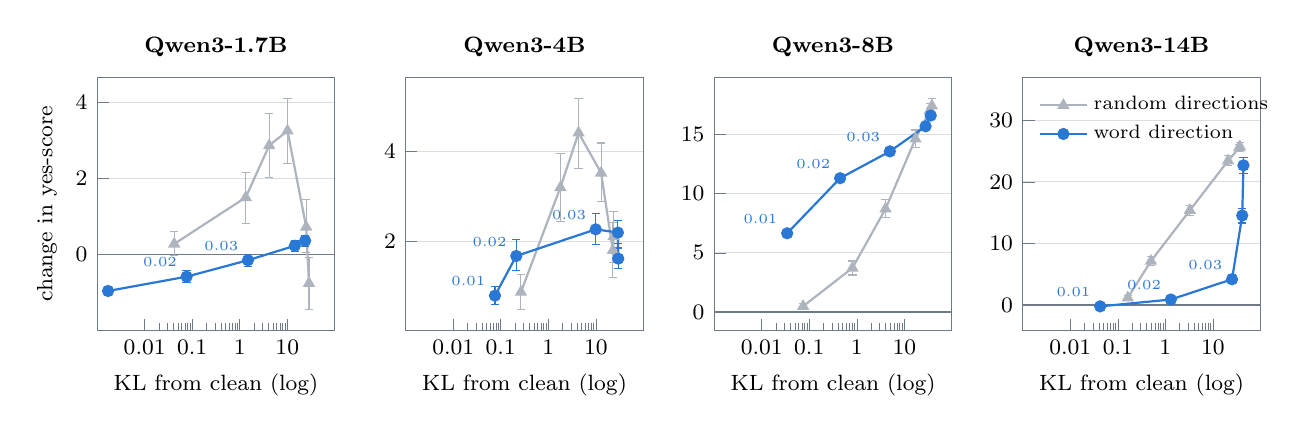
\begin{tikzpicture}
\begin{groupplot}[group style={group size=4 by 1, horizontal sep=0.9cm}, width=4.6cm, height=4.8cm, xmode=log,
  xmin=0.001, xmax=100, xtick={0.01,0.1,1,10}, xticklabels={0.01,0.1,1,10}, xlabel={KL from clean (log)}, legend cell align=left]
\nextgroupplot[title={Qwen3-1.7B}, ylabel={change in yes-score}, ]
\draw[cGrey, line width=0.5pt] (axis cs:0.001,0) -- (axis cs:100,0);
\addplot[color=cLight, mark=triangle*, mark size=1.8pt, line width=0.8pt, err] coordinates {(0.0418,0.28229) += (0,0.32187) -= (0,0.30000) (1.3376,1.50156) += (0,0.64948) -= (0,0.68594) (4.1675,2.86146) += (0,0.84792) -= (0,0.83438) (10.1237,3.24661) += (0,0.85091) -= (0,0.85664) (25.0230,0.72729) += (0,0.71286) -= (0,0.66972) (28.6385,-0.74779) += (0,0.68184) -= (0,0.68887)};

\addplot[color=cA, mark=*, mark size=1.8pt, line width=0.8pt, err] coordinates {(0.0017,-0.95000) += (0,0.11875) -= (0,0.11875) (0.0764,-0.57500) += (0,0.16250) -= (0,0.15937) (1.4910,-0.14375) += (0,0.15000) -= (0,0.15937) (14.4108,0.23438) += (0,0.14375) -= (0,0.15000) (23.7540,0.36562) += (0,0.14062) -= (0,0.14375)};

\node[font=\tiny, color=cA, anchor=south east] at (axis cs:0.0017,-0.9500) {0.01};
\node[font=\tiny, color=cA, anchor=south east] at (axis cs:0.0764,-0.5750) {0.02};
\node[font=\tiny, color=cA, anchor=south east] at (axis cs:1.4910,-0.1437) {0.03};
\nextgroupplot[title={Qwen3-4B}, ]
\draw[cGrey, line width=0.5pt] (axis cs:0.001,0) -- (axis cs:100,0);
\addplot[color=cLight, mark=triangle*, mark size=1.8pt, line width=0.8pt, err] coordinates {(0.2662,0.87292) += (0,0.39375) -= (0,0.38750) (1.7985,3.19010) += (0,0.75885) -= (0,0.76302) (4.3462,4.40234) += (0,0.76302) -= (0,0.78542) (12.9506,3.51276) += (0,0.66393) -= (0,0.63678) (22.8403,1.79641) += (0,0.62686) -= (0,0.61007) (23.6959,2.10553) += (0,0.54813) -= (0,0.56982)};

\addplot[color=cA, mark=*, mark size=1.8pt, line width=0.8pt, err] coordinates {(0.0756,0.79375) += (0,0.20000) -= (0,0.18750) (0.2124,1.67188) += (0,0.36563) -= (0,0.32812) (9.9758,2.26250) += (0,0.34375) -= (0,0.33438) (29.1673,2.19062) += (0,0.26562) -= (0,0.24687) (29.6872,1.61406) += (0,0.23438) -= (0,0.22344)};

\node[font=\tiny, color=cA, anchor=south east] at (axis cs:0.0756,0.7937) {0.01};
\node[font=\tiny, color=cA, anchor=south east] at (axis cs:0.2124,1.6719) {0.02};
\node[font=\tiny, color=cA, anchor=south east] at (axis cs:9.9758,2.2625) {0.03};
\nextgroupplot[title={Qwen3-8B}, ]
\draw[cGrey, line width=0.5pt] (axis cs:0.001,0) -- (axis cs:100,0);
\addplot[color=cLight, mark=triangle*, mark size=1.8pt, line width=0.8pt, err] coordinates {(0.0742,0.48542) += (0,0.25938) -= (0,0.27500) (0.8108,3.72396) += (0,0.58698) -= (0,0.59271) (4.0313,8.71875) += (0,0.80469) -= (0,0.76094) (17.1441,14.62479) += (0,0.75160) -= (0,0.75047) (34.5554,17.03698) += (0,0.58718) -= (0,0.60937) (38.0896,17.41043) += (0,0.63363) -= (0,0.63327)};

\addplot[color=cA, mark=*, mark size=1.8pt, line width=0.8pt, err] coordinates {(0.0343,6.65000) += (0,0.19687) -= (0,0.20625) (0.4452,11.30313) += (0,0.13125) -= (0,0.14531) (4.9642,13.56719) += (0,0.12656) -= (0,0.12656) (27.9896,15.68594) += (0,0.12188) -= (0,0.12344) (35.9216,16.59375) += (0,0.12031) -= (0,0.12187)};

\node[font=\tiny, color=cA, anchor=south east] at (axis cs:0.0343,6.6500) {0.01};
\node[font=\tiny, color=cA, anchor=south east] at (axis cs:0.4452,11.3031) {0.02};
\node[font=\tiny, color=cA, anchor=south east] at (axis cs:4.9642,13.5672) {0.03};
\nextgroupplot[title={Qwen3-14B}, legend pos=north west, ymax=37,]
\draw[cGrey, line width=0.5pt] (axis cs:0.001,0) -- (axis cs:100,0);
\addplot[color=cLight, mark=triangle*, mark size=1.8pt, line width=0.8pt, err] coordinates {(0.1621,1.18021) += (0,0.30781) -= (0,0.27604) (0.4981,7.13672) += (0,0.68542) -= (0,0.66979) (3.2778,15.37591) += (0,0.82383) -= (0,0.85924) (20.8643,23.43385) += (0,0.83122) -= (0,0.81142) (35.8170,25.53522) += (0,0.59634) -= (0,0.55255) (36.9658,25.73888) += (0,0.59469) -= (0,0.58401)};
\addlegendentry{random directions}
\addplot[color=cA, mark=*, mark size=1.8pt, line width=0.8pt, err] coordinates {(0.0426,-0.21250) += (0,0.18906) -= (0,0.20469) (1.3061,0.89844) += (0,0.45156) -= (0,0.46094) (25.2952,4.18906) += (0,0.82500) -= (0,0.73594) (41.4829,14.54141) += (0,1.19609) -= (0,1.21719) (43.9868,22.68740) += (0,1.26025) -= (0,1.28301)};
\addlegendentry{word direction}
\node[font=\tiny, color=cA, anchor=south east] at (axis cs:0.0426,-0.2125) {0.01};
\node[font=\tiny, color=cA, anchor=south east] at (axis cs:1.3061,0.8984) {0.02};
\node[font=\tiny, color=cA, anchor=south east] at (axis cs:25.2952,4.1891) {0.03};
\end{groupplot}
\end{tikzpicture}
\end{document}
